\begin{figure}[htb]
\centering
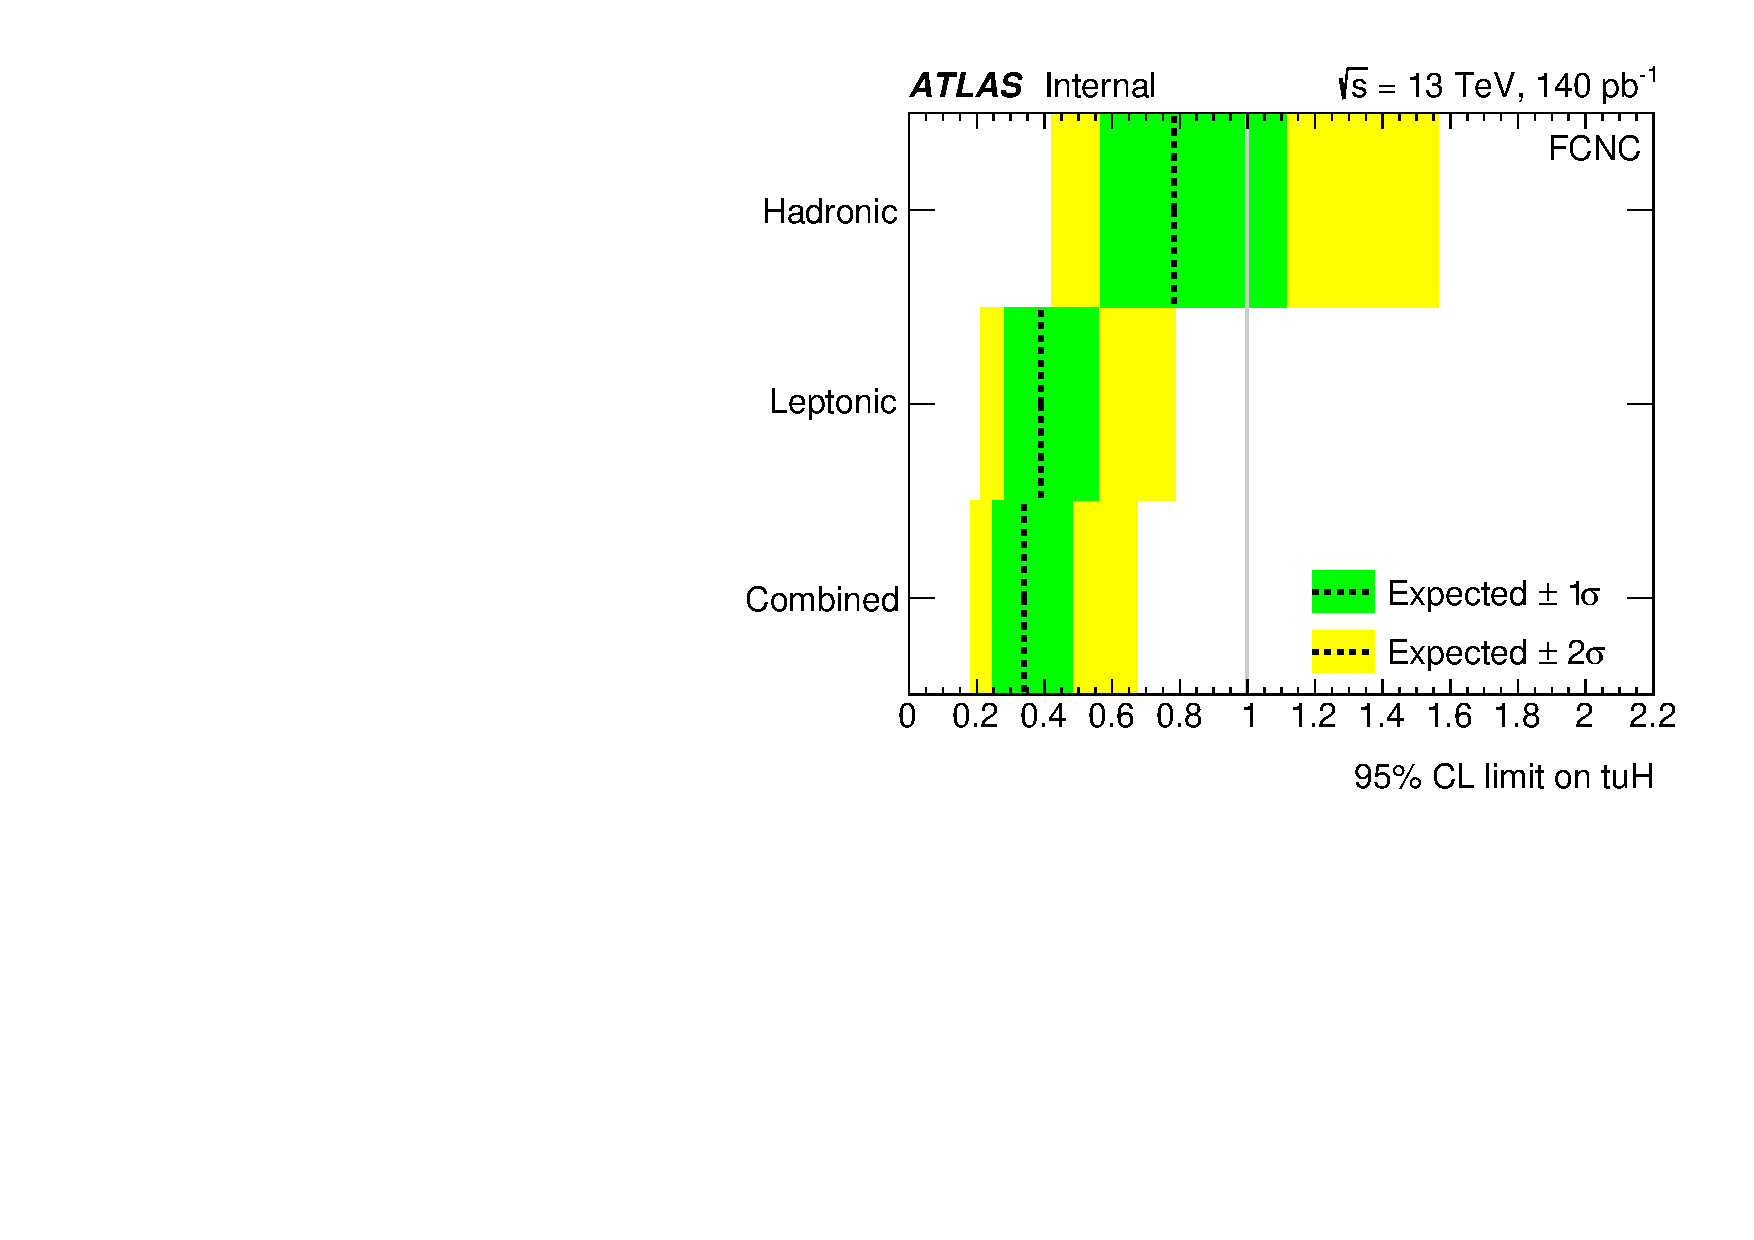
\includegraphics[width=0.48\textwidth]{\FCNCFigures/tuH_combined_Limit.pdf}
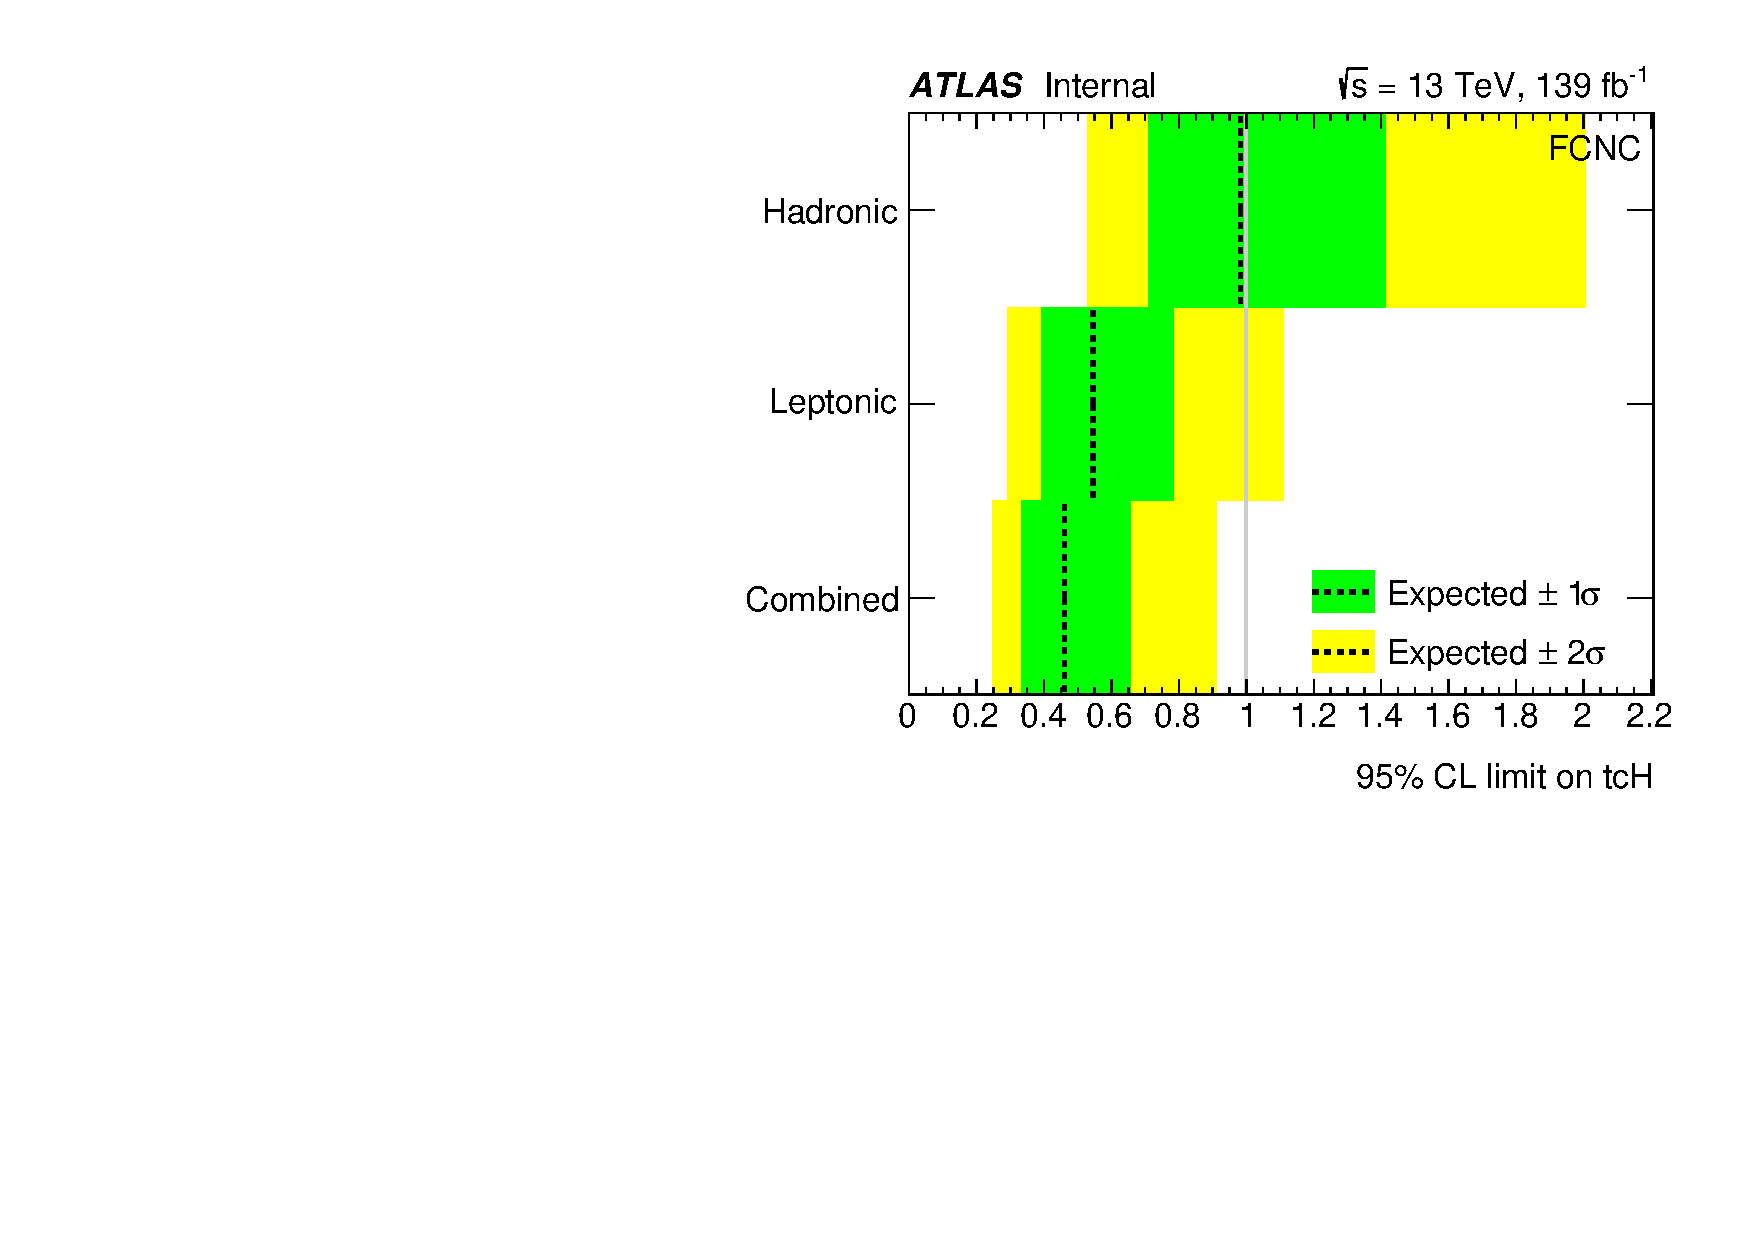
\includegraphics[width=0.48\textwidth]{\FCNCFigures/tcH_combined_Limit.pdf}
%\put(-50, 150){\textbf{(a)}}
\caption{95\% CL upper limits on B($t\rightarrow Hu$) versus B($t\rightarrow Hc$) for the individual channel as well as their combination. %The observed limits (solid lines) are compared with 
The expected (median) limits under the background-only hypothesis is shown in dotted lines. The surrounding shaded bands correspond to the 68\% and 95\% CL
intervals around the expected limits, denoted by $\pm1\sigma$ and $\pm2\sigma$, respectively. }
\label{fig:combined_limit}
\end{figure}

\begin{figure}[htb]
\centering
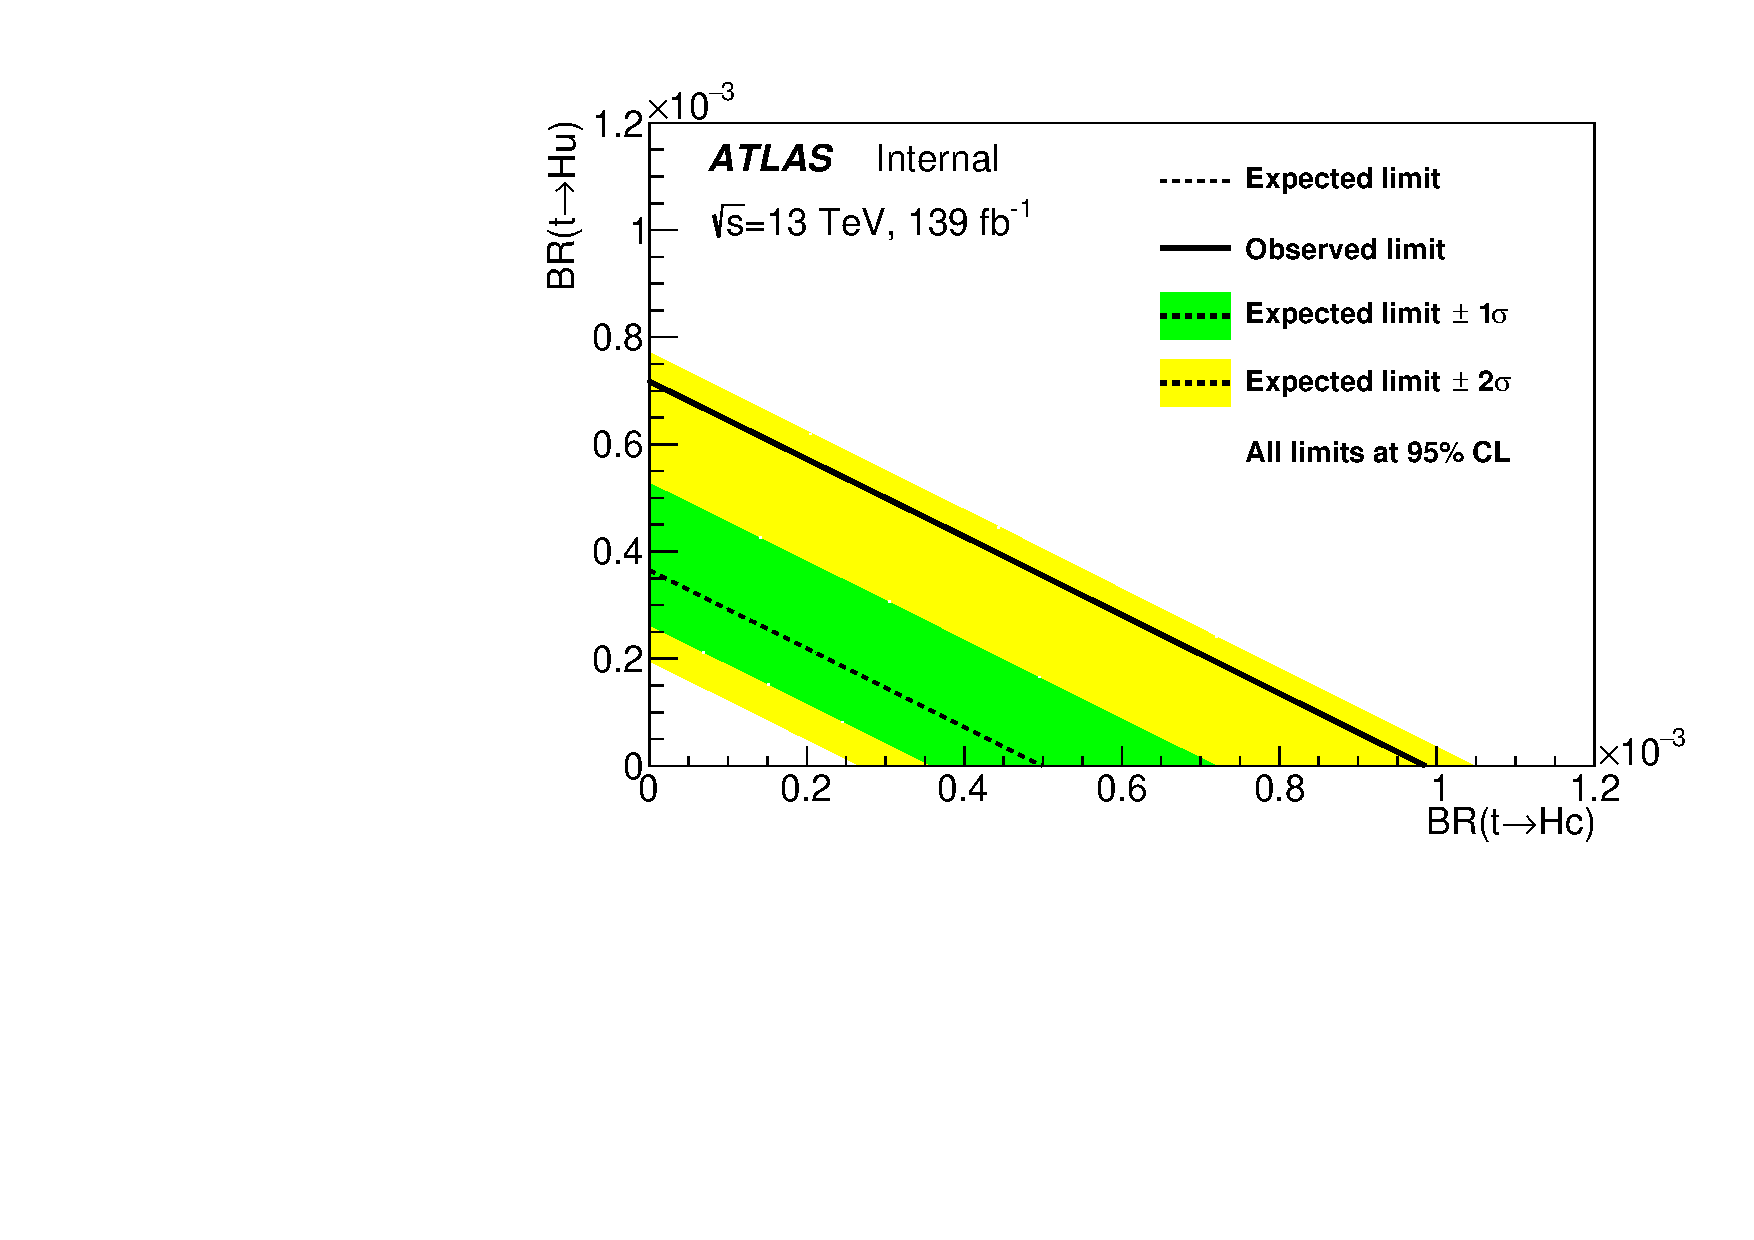
\includegraphics[width=0.48\textwidth]{\FCNCFigures/2DLimits.pdf}
\caption{95\% CL upper limits on the plane of B($t\rightarrow Hu$) versus B($t\rightarrow Hc$) for the combination of the searches. The expected
(median) limits under the background-only hypothesis is shown in dotted lines. The surrounding shaded bands correspond to
the 68\% and 95\% CL intervals around the expected limits, denoted by $\pm1\sigma$ and $\pm2\sigma$, respectively.}
\label{fig:combined_limit}
\end{figure}